\chapter{Methodology}
\label{ch:methodology}

\section{Introduction}
\label{sec:meth-intro}

This chapter presents the complete engineering methodology behind NirmalNode: the overall system architecture; the hardware used at the sensing and purification layers; the software running on the microcontroller; the communication and cloud architecture that connects the physical node to the AI layer; the Adaptive AI pipeline, including the mathematical formulation of the incremental-learning models used; and the decision logic that converts a pollution forecast into a physical purifier action. Each subsystem is described with enough implementation detail (equations, pseudocode, and architecture diagrams) to be reproducible.

\section{System Overview}
\label{sec:meth-overview}

NirmalNode is organized into five functional layers, illustrated in Figure~\ref{fig:five-layer}: (1) Environmental Monitoring, where physical sensors sample the air at the hotspot; (2) IoT Data Acquisition, where the ESP32 reads, cleans, timestamps, and transmits sensor data; (3) Cloud Data Storage, where historical and streaming data are persisted; (4) Adaptive AI Prediction, where an incrementally-updated model forecasts pollution 1--2 hours ahead; and (5) Local Air Purification, where the physical cyclone--HEPA--activated-carbon unit is triggered in response to the prediction.

\begin{figure}[htbp]
\centering
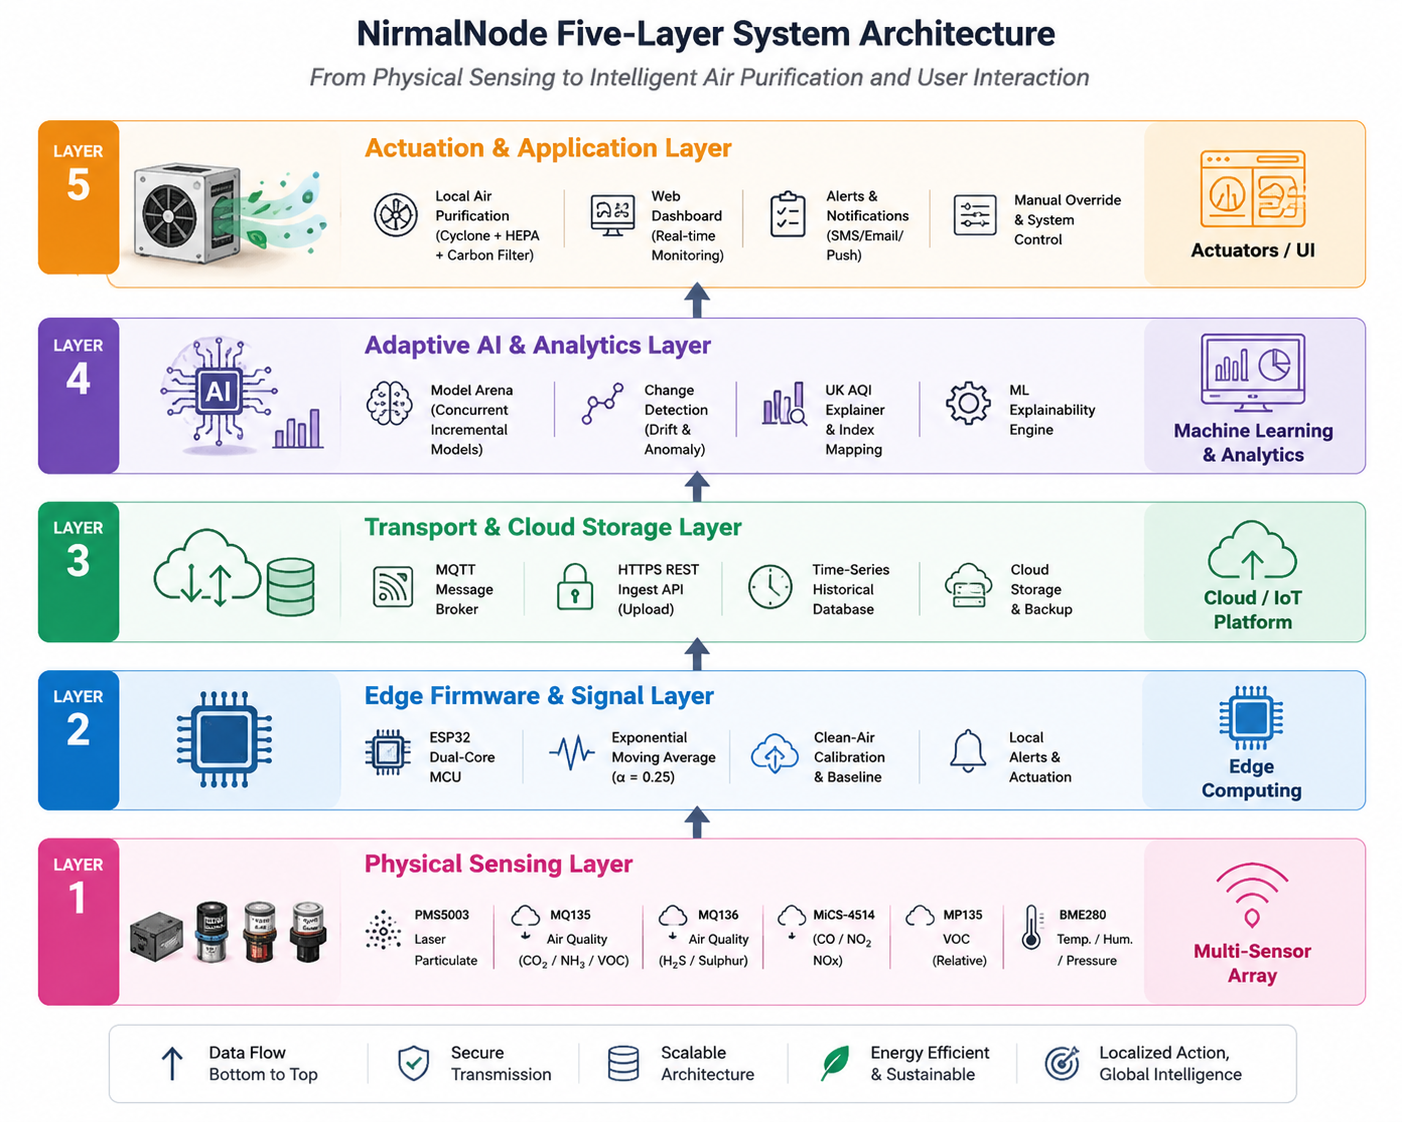
\includegraphics[width=0.92\textwidth]{figures/five_layer_architecture.png}
\caption{Five-layer system architecture of NirmalNode.}
\label{fig:five-layer}
\end{figure}

\section{System Flow}
\label{sec:meth-system-flow}

At a fixed sampling interval $\Delta t$ (prototype value: $\Delta t = 60$~s), the ESP32 reads all connected sensors, applies noise filtering, appends a timestamp and location identifier, and transmits the resulting record to the cloud database over Wi-Fi. The cloud layer appends the record to the historical dataset and forwards it to the Adaptive AI module, which produces two outputs: (a) an incremental update to its internal model parameters using the newly arrived data point, and (b) a forecast of pollutant concentration at time $t+h$ (with $h \in [1,2]$ hours). The forecast is passed to a threshold-based Decision Engine, which activates the purifier fan if the forecast crosses a hazard threshold, allowing purification to begin \emph{before} the hazardous condition materializes. Figure~\ref{fig:workflow} shows the complete, end-to-end workflow.

\begin{figure}[htbp]
\centering
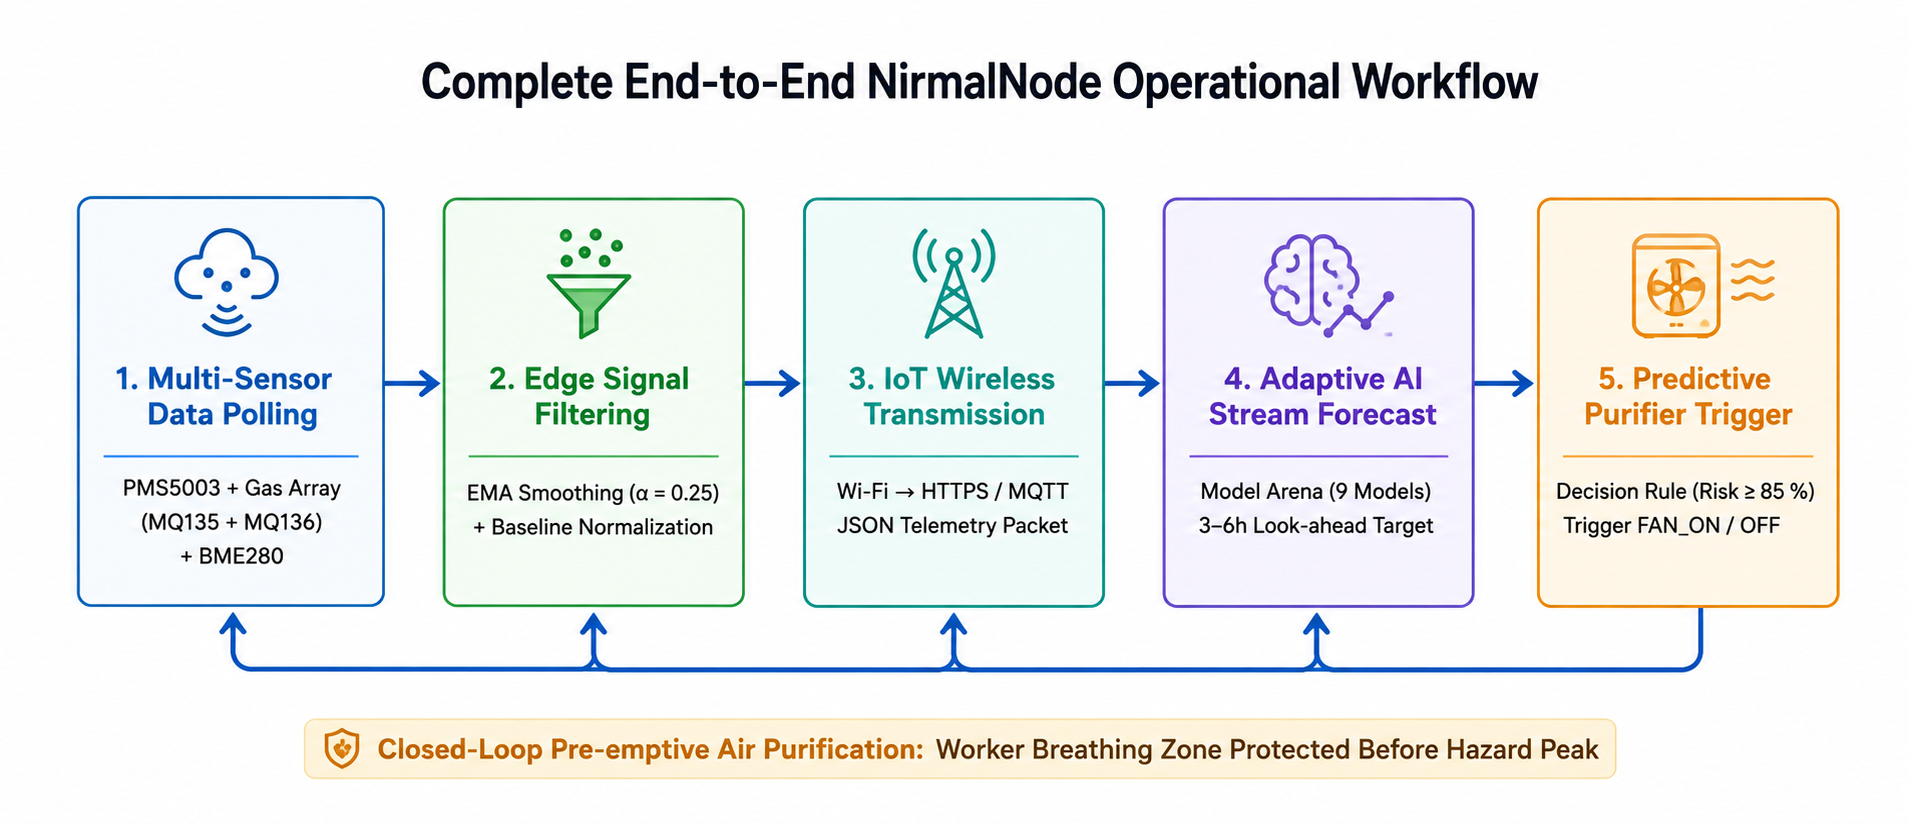
\includegraphics[width=\textwidth]{figures/system_workflow.png}
\caption{Complete end-to-end system workflow, from sensing to clean-air delivery.}
\label{fig:workflow}
\end{figure}

\FloatBarrier

\section{Hardware Architecture}
\label{sec:meth-hardware}

\subsection{ESP32 Microcontroller (Central Controller)}
\label{sec:meth-esp32}

The ESP32 Dev Module is used as the central controller of each NirmalNode unit. Its responsibilities are: (i) polling all attached sensors at the sampling interval $\Delta t$; (ii) applying a noise-filtering stage (Section~\ref{sec:meth-filtering}) to each raw reading; (iii) generating a timestamp and attaching the fixed location identifier of the node; (iv) formatting the resulting record (e.g., as JSON) for transmission; (v) transmitting the record to the cloud layer over Wi-Fi; (vi) receiving the prediction/decision result back from the cloud (or computing it locally, in an edge-AI configuration); and (vii) driving the purifier fan relay accordingly. The ESP32 was selected over alternative microcontrollers because it offers built-in Wi-Fi, multiple analog-to-digital converter (ADC) channels (needed for the analog gas sensors), UART interfaces (needed for the PMS5003's digital serial output), sufficiently high processing speed for on-device filtering and, where required, lightweight inference, low unit cost, low power consumption suitable for battery operation, and strong community/library support -- all of which directly support the Green IoT design goal of Section~\ref{sec:lr-green}.

\subsection{PMS5003 -- Laser Particulate Matter Sensor}
The PMS5003 is a laser-scattering particulate sensor that reports mass concentrations of PM1.0, PM2.5, and PM10. Air is drawn through an internal sensing chamber by a small fan; particles suspended in the air scatter a laser beam, and an internal photodiode measures the intensity and pattern of scattered light, from which the sensor's onboard processor estimates particle count and size distribution, and in turn mass concentration. PM2.5 is the single most safety-critical channel reported by this sensor, since particles below 2.5~$\mu$m are small enough to penetrate deep into the alveolar region of the lungs, which is the physiological basis for the health outcomes reviewed in Section~\ref{sec:lr-occupational-health}.

\subsection{MQ135 -- General Air Quality / Gas Sensor}
The MQ135 is a metal-oxide semiconductor (MOS) gas sensor whose resistance changes in the presence of a broad range of gases, including VOCs, smoke, NH$_3$, NO$_x$, alcohol vapour, and benzene, and which can additionally provide an indirect, non-quantitative estimate of elevated CO$_2$. Because it is a broad-spectrum sensor rather than a gas-specific one, its output is used in NirmalNode as a general air-quality indicator feature rather than as a calibrated single-gas concentration channel.

\subsection{MQ136 -- Hydrogen Sulphide Sensor}
The MQ136 is a MOS sensor specialized for hydrogen sulphide (H$_2$S) detection. H$_2$S is of particular concern in chemical processing, tanning/leather, waste-treatment, and food-processing industries -- all common in the Bangladeshi industrial landscape -- and is acutely toxic at elevated concentrations, motivating its inclusion as a dedicated sensing channel rather than relying on the broad-spectrum MQ135 alone.

\subsection{MiCS-4514 -- Dual-Element Gas Sensor}
The MiCS-4514 integrates two independent MOS sensing elements on a single package: a \emph{RED} element sensitive to carbon monoxide, hydrogen, methane, ethanol, and ammonia, and an \emph{OX} element sensitive to nitrogen dioxide. Because CO and NO$_2$ are both primary combustion by-products expected at boiler-room and generator-room hotspots, and because the two elements can be sampled simultaneously and independently, this sensor allows NirmalNode to monitor multiple industrially relevant gases from a single compact component.

\subsection{MP135 -- Supplementary Air Quality Sensor}
The MP135 provides a further general-purpose air-quality indication and is used to complement the MQ135 channel. Using multiple, partially overlapping gas sensors improves the robustness of the overall gas-sensing subsystem, since individual MOS sensors differ in their sensitivity range, response time, and cross-sensitivity to interfering gases; combining several sensors' outputs as separate input features allows the downstream AI model (Section~\ref{sec:meth-ai-pipeline}) to implicitly learn to weight and combine them appropriately for the specific hotspot in which the unit is deployed.

\subsection{BME280 (Optional) -- Temperature, Humidity, and Pressure}
An optional BME280 sensor provides ambient temperature, relative humidity, and atmospheric pressure readings. These environmental variables are included as AI input features because pollutant dispersion, particulate suspension, and gas-sensor response are all known to be modulated by temperature and humidity, and because diurnal pressure/temperature cycles correlate with certain industrial activity patterns (e.g., process heat cycles). The baseline environmental compensation applied across sensor channels is defined as:
\begin{equation}
C_{\text{compensated}} = C_{\text{raw}} \cdot \Big(1 - \alpha (T - T_{\text{ref}}) - \beta (RH - RH_{\text{ref}})\Big)
\label{eq:corr}
\end{equation}
where $T_{\text{ref}} = 20^\circ\text{C}$, $RH_{\text{ref}} = 65\%$, and $\alpha, \beta$ denote the sensor-specific temperature and humidity compensation coefficients.

\subsection{Power Supply}
The bench-scale prototype is powered by a laboratory DC power supply for ease of development and testing. The design target for field deployment is a Lithium-Polymer (Li-Po) battery, selected to make the unit portable and independent of a fixed mains connection, which is important for retrofitting hotspots in existing factory floors where wiring a new mains-powered appliance may be impractical or unsafe.

\begin{table}[htbp]
\centering
\caption{Hardware components used in the NirmalNode prototype}
\label{tab:hardware-components}
\small
\begin{tabular}{@{}p{3.4cm}p{5.2cm}p{5.2cm}@{}}
\toprule
\textbf{Component} & \textbf{Function} & \textbf{Measured / Controlled Quantity} \\
\midrule
ESP32 Dev Module & Central controller & Sensor polling, filtering, communication, purifier control \\
PMS5003 & Laser particulate sensor & PM1.0, PM2.5, PM10 \\
MQ135 & General gas sensor & VOC, smoke, NH$_3$, NO$_x$, alcohol, benzene (indicative CO$_2$) \\
MQ136 & Specialized gas sensor & H$_2$S \\
MiCS-4514 & Dual-element gas sensor & CO, H$_2$, CH$_4$, ethanol, NH$_3$ (RED); NO$_2$ (OX) \\
MP135 & Supplementary gas sensor & General air-quality indication \\
BME280 (optional) & Environmental sensor & Temperature, humidity, pressure \\
DC Fan & Air mover & Draws air through the purification chamber \\
Cyclone Separator & Coarse pre-filter & Removes large dust particles \\
HEPA Filter & Fine particulate filter & PM2.5, PM1.0, dust, smoke, pollen, microorganisms \\
Activated Carbon Filter & Gas/odour filter & VOC, odour, organic gases, chemical vapours \\
Bench DC Supply / Li-Po Battery & Power source & Prototype bench power / portable field power \\
\bottomrule
\end{tabular}
\end{table}

\FloatBarrier

\section{Purification Subsystem}
\label{sec:meth-purification}

\subsection{Cyclone Separator}
The cyclone separator is the first purification stage. Polluted air enters the separator tangentially, and the resulting swirling flow subjects suspended particles to a centrifugal force
\begin{equation}
F_c = \frac{m\,v_t^2}{r}
\label{eq:centrifugal}
\end{equation}
where $m$ is particle mass, $v_t$ is the tangential velocity of the swirling air, and $r$ is the radius of the swirl path. Larger, heavier particles experience a proportionally larger $F_c$ and are thrown toward the outer wall of the separator, from which they fall into a dust-collection chamber, while the (now coarse-particle-depleted) air stream continues to the HEPA stage. This pre-separation step reduces the particulate loading reaching the HEPA filter, extending its usable lifetime.

\subsection{HEPA Filter}
The HEPA filter stage removes fine particulate matter, including PM2.5, PM1.0, residual dust, smoke particles, pollen, and many microorganisms. Filtration performance is conventionally expressed as a removal efficiency
\begin{equation}
\eta = 1 - \frac{C_{\text{out}}}{C_{\text{in}}}
\label{eq:hepa-efficiency}
\end{equation}
where $C_{\text{in}}$ and $C_{\text{out}}$ are the pollutant mass concentrations upstream and downstream of the filter, respectively. A filter meeting the HEPA standard achieves $\eta \geq 0.9997$ (i.e., at least 99.97\% removal) for particles of the most penetrating size, approximately 0.3~$\mu$m in diameter.

\subsection{Activated Carbon Filter}
The activated carbon stage removes gaseous pollutants -- VOCs, odour-causing compounds, and other organic/chemical vapours -- that pass through the HEPA stage unaffected, via physical adsorption onto the very large internal pore surface area of activated carbon. Adsorption capacity as a function of gas-phase concentration at equilibrium is commonly described by the Langmuir isotherm,
\begin{equation}
q_e = \frac{q_{\max} K C_e}{1 + K C_e}
\label{eq:langmuir}
\end{equation}
where $q_e$ is the mass of pollutant adsorbed per unit mass of carbon at equilibrium, $C_e$ is the equilibrium gas-phase concentration, $q_{\max}$ is the maximum adsorption capacity of the carbon, and $K$ is the Langmuir adsorption constant. This relationship is used qualitatively in this thesis to motivate periodic replacement of the activated-carbon cartridge as its effective $q_{\max}$ is approached, rather than as a fitted quantitative model (fitting Equation~\ref{eq:langmuir} to the specific carbon medium used is left as a calibration task; see Chapter 4, Limitations).

\subsection{Purification Pipeline}
Figure~\ref{fig:purification-pipeline} shows the physical purification pipeline in isolation, corresponding to Layer 5 of Figure~\ref{fig:five-layer}.

\begin{figure}[htbp]
\centering
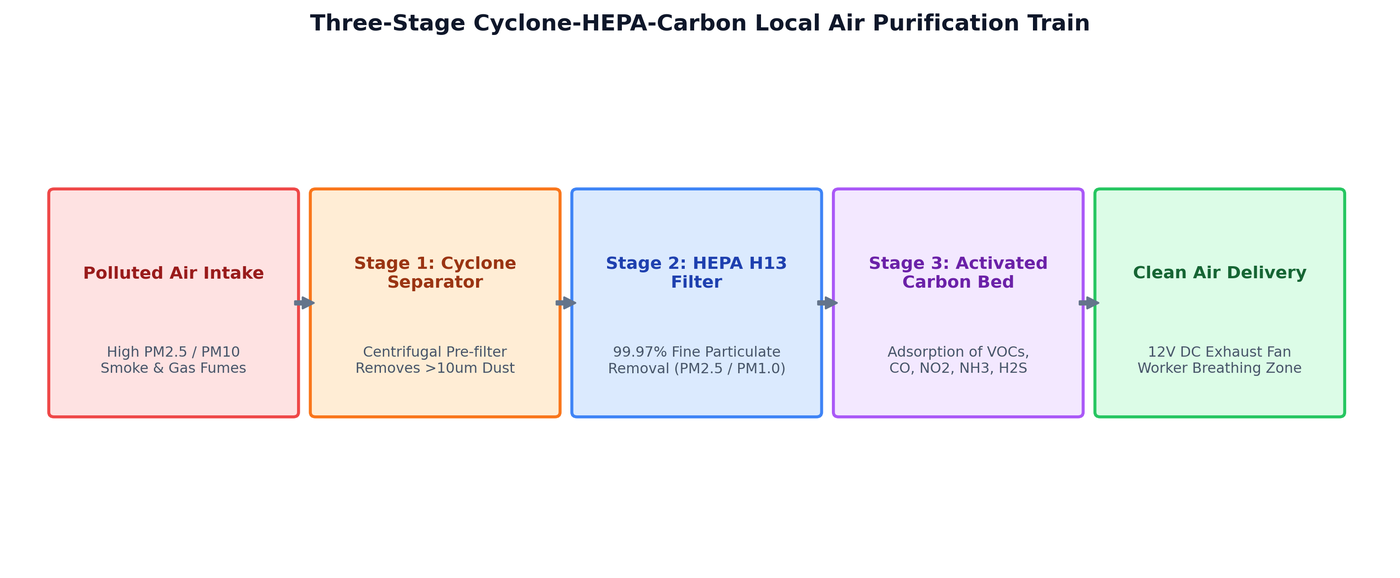
\includegraphics[width=\textwidth]{figures/purification_pipeline.png}
\caption{Three-stage cyclone-HEPA-carbon local air purification train.}
\label{fig:purification-pipeline}
\end{figure}

\FloatBarrier

\section{Software Architecture and Sensor Filtering}
\label{sec:meth-software}

\subsection{Noise Filtering}
\label{sec:meth-filtering}
Raw MOS gas-sensor readings are known to be noisy and drift-prone. Each raw reading $x_{\text{raw}}[k]$ at sample index $k$ is smoothed on-device using an exponential moving average (EMA),
\begin{equation}
\hat{x}[k] = \alpha\, x_{\text{raw}}[k] + (1-\alpha)\, \hat{x}[k-1]
\label{eq:ema}
\end{equation}
where $\alpha \in (0,1]$ is a smoothing constant chosen to trade off responsiveness against noise suppression (a higher $\alpha$ tracks rapid pollution changes more closely; a lower $\alpha$ suppresses more sensor noise). The filtered value $\hat{x}[k]$, rather than the raw reading, is used for both cloud transmission and AI model input.

\subsection{ESP32 Firmware Logic}
Algorithm~\ref{alg:esp32-loop} summarizes the main firmware loop executed on the ESP32.

\begin{algorithm}[htbp]
\caption{ESP32 Main Sensing and Transmission Loop}
\label{alg:esp32-loop}
\begin{algorithmic}[1]
\State Initialize Wi-Fi connection, sensor interfaces, and EMA state $\hat{x} \leftarrow 0$
\Loop
    \State Read raw values from PMS5003, MQ135, MQ136, MiCS-4514, MP135, BME280
    \For{each sensor channel $x_{\text{raw}}$}
        \State $\hat{x} \leftarrow \alpha\, x_{\text{raw}} + (1-\alpha)\, \hat{x}$ \Comment{EMA filtering, Eq.~\ref{eq:ema}}
    \EndFor
    \State Generate timestamp $t$ and attach fixed location ID
    \State Assemble record $r = \{\hat{x}_{\text{PM1.0..PM10}}, \hat{x}_{\text{CO,NO}_2}, \hat{x}_{\text{VOC,NH}_3,\text{H}_2\text{S}}, \hat{x}_{T,H,P}, t, \text{locationID}\}$ \Comment{full feature set, Eq.~\ref{eq:feature-vector}}
    \State Transmit $r$ to Cloud Database over Wi-Fi
    \State Receive Decision Engine output $d \in \{\text{ON}, \text{OFF}\}$ from cloud (or compute locally at the edge)
    \State Set purifier relay state according to $d$
    \State Sleep for sampling interval $\Delta t$
\EndLoop
\end{algorithmic}
\end{algorithm}

\FloatBarrier

\section{Communication and Cloud Architecture}
\label{sec:meth-cloud}

\subsection{Communication Architecture}
Each NirmalNode unit communicates with the cloud layer over Wi-Fi using a lightweight, JSON-formatted payload sent either via HTTPS POST requests or an MQTT publish to a node-specific topic (e.g., \texttt{nirmalnode/<locationID>/telemetry}). MQTT is preferred where available because its publish/subscribe model and small message overhead further support the Green IoT objective of minimizing communication energy cost, and because it naturally supports the Decision Engine subscribing to, and acting on, the same telemetry stream in near real time.

\subsection{Cloud Data Architecture}
The cloud layer maintains a time-series database in which every record is keyed by (\texttt{location\_id}, \texttt{timestamp}) and stores the full feature vector described in Section~\ref{sec:meth-data-pipeline}. This store serves three purposes: (i) it is the historical dataset from which the initial AI model (Section~\ref{sec:meth-ai-pipeline}) is trained; (ii) it is the source of the continuous stream of new records used for incremental model updates; and (iii) it supports a monitoring dashboard for human oversight of both raw pollutant levels and model predictions. Figure~\ref{fig:cloud-arch} depicts this architecture.

\begin{figure}[htbp]
    \centering
    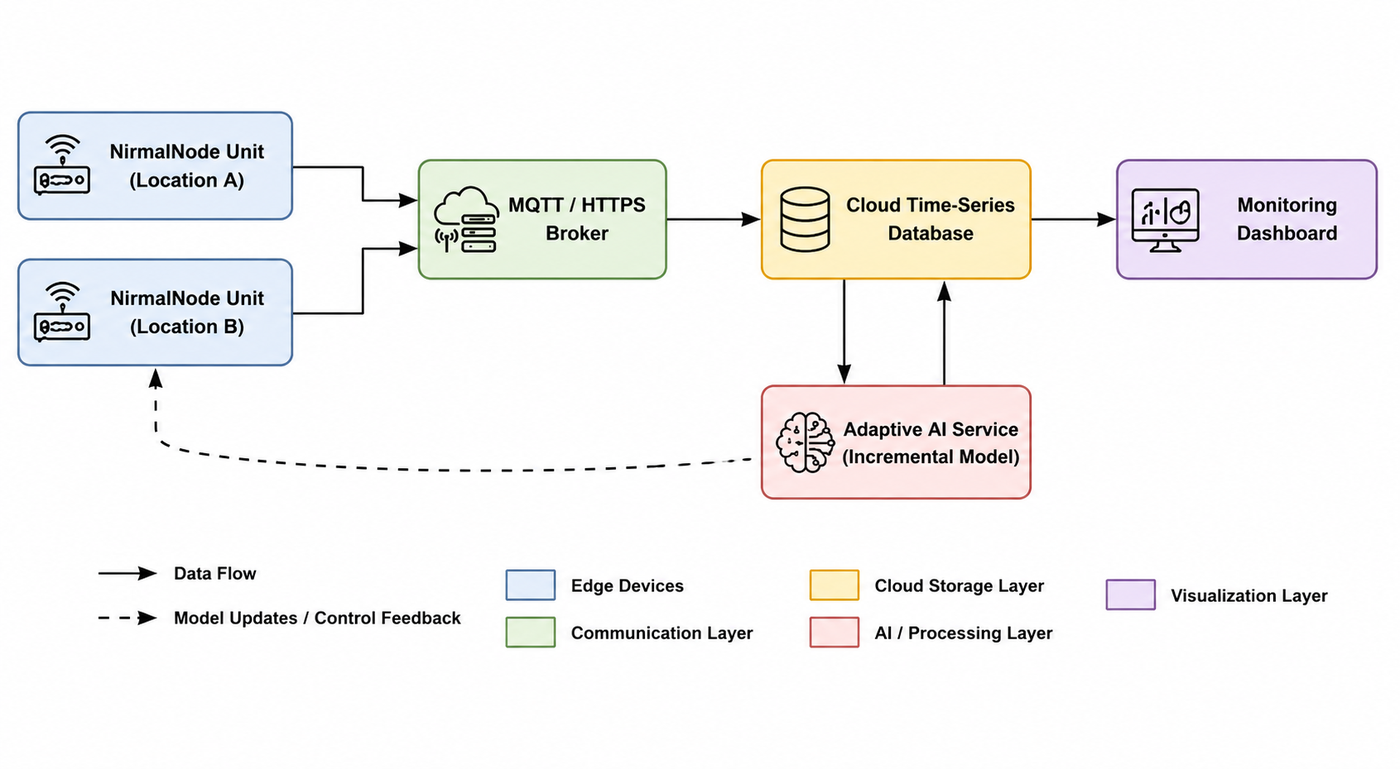
\includegraphics[width=\textwidth]{figures/edge_cloud_architecture.png}
    \caption{Edge--cloud communication and data architecture (illustrated for two deployed units).}
    \label{fig:cloud-arch}
\end{figure}

\FloatBarrier

\section{Data Pipeline and Feature Definition}
\label{sec:meth-data-pipeline}

Table~\ref{tab:features} lists the complete AI input feature vector, and Table~\ref{tab:ai-output} lists the AI output variables. At each sampling instant $t$, the feature vector is
\begin{equation}
\small
\begin{aligned}
\mathbf{x}_t = \big[\, &\text{PM1.0}_t,\ \text{PM2.5}_t,\ \text{PM10}_t,\ \text{CO}_t,\ \text{NO}_{2,t},\ \text{VOC}_t,\ \text{NH}_{3,t},\ \text{H}_2\text{S}_t, \\
&T_t,\ H_t,\ P_t,\ \text{hour}_t,\ \text{day}_t,\ y_{t-1} \,\big]
\end{aligned}
\label{eq:feature-vector}
\end{equation}
where $y_{t-1}$ is the previous observed pollution level (e.g., PM2.5 or a composite index), included so that the model can exploit short-term temporal autocorrelation in pollution levels in addition to the instantaneous multi-sensor reading.

\begin{table}[htbp]
\centering
\caption{AI input feature set}
\label{tab:features}
\small
\begin{tabular}{@{}p{4.5cm}p{8cm}@{}}
\toprule
\textbf{Feature} & \textbf{Description} \\
\midrule
PM1.0, PM2.5, PM10 & Particulate matter mass concentration (from PMS5003) \\
CO, NO$_2$ & Combustion-related gas concentration (from MiCS-4514) \\
VOC, NH$_3$ & Volatile organic compounds and ammonia (from MQ135 / MiCS-4514) \\
H$_2$S & Hydrogen sulphide (from MQ136) \\
Temperature, Humidity, Pressure & Ambient environmental conditions (from BME280) \\
Hour of Day & Cyclical feature capturing diurnal industrial activity patterns \\
Day of Week & Captures weekly production-schedule patterns \\
Previous Pollution Level ($y_{t-1}$) & Short-term temporal autocorrelation feature \\
\bottomrule
\end{tabular}
\end{table}

\begin{table}[htbp]
\centering
\caption{AI output variables}
\label{tab:ai-output}
\small
\begin{tabular}{@{}p{4.5cm}p{8cm}@{}}
\toprule
\textbf{Output} & \textbf{Description} \\
\midrule
Predicted pollution level $\hat{y}_{t+h}$ & Forecast pollutant concentration $h \in [1,2]$ hours ahead \\
Predicted AQI category & Discretized air-quality-index class derived from $\hat{y}_{t+h}$ \\
Risk level & Low / Moderate / High / Hazardous classification \\
Purifier recommendation & Binary decision (Activate / Do not activate) passed to the Decision Engine \\
\bottomrule
\end{tabular}
\end{table}

\FloatBarrier

\section{Adaptive AI Pipeline}
\label{sec:meth-ai-pipeline}

\subsection{Initial (Offline) Training}
Prior to field deployment, an initial model $f(\cdot\,;\mathbf{w}_0)$ is trained in batch mode on a historical Bangladesh air-quality dataset, using standard supervised regression, to obtain a reasonable starting parameter vector $\mathbf{w}_0$. This offline stage exists purely to give the deployed unit a sensible initial state; it is not repeated after deployment.

\subsection{Incremental (Online) Learning and the Model Arena}
After deployment, the forecasting module operates under the \emph{prequential (test-then-train)} protocol. Rather than relying on a single static model, NirmalNode implements a competitive multi-model tournament framework termed the \textbf{Model Arena}. In the Model Arena, nine diverse incremental models run concurrently on the incoming stream. Each sample $\mathbf{x}_t$ is first evaluated to score each model's prior prediction, after which all nine models are incrementally updated via \texttt{partial\_fit()}. Once a warm-up phase of $N_{\text{warmup}} = 50$ samples is completed, the Arena automatically elects the model with the minimum cumulative prequential MAE as the active production champion ($M_{\text{champion}}$) driving the purifier actuator.

The nine candidate models spanning varied loss functions, regularizers, and update rules are:
\begin{enumerate}[label=\textbf{M\arabic*:},leftmargin=*]
    \item \textbf{SGD Regressor (Squared Error, $L_2$ Regularization -- Ridge Online):} Minimizes standard MSE with $L_2$ penalty:
    \begin{equation}
    \mathbf{w}_{t+1} = (1 - \eta_t \alpha)\mathbf{w}_t - \eta_t (f(\mathbf{x}_t;\mathbf{w}_t) - y_t)\mathbf{x}_t
    \label{eq:sgd}
    \end{equation}
    \item \textbf{SGD Regressor (Squared Error, $L_1$ Regularization -- Lasso Online):} Uses $L_1$ penalty to induce feature sparsity during stream adaptation.
    \item \textbf{SGD Regressor (ElasticNet):} Blends $L_1$ and $L_2$ penalties ($\rho = 0.5$) for balanced regularisation in the presence of correlated gas sensor channels.
    \item \textbf{SGD Regressor (Huber Loss, $L_2$ Regularization):} Employs the robust Huber loss with threshold $\delta = 1.35$:
    \begin{equation}
    \mathcal{L}_{\delta}(e) = \begin{cases} \frac{1}{2}e^2, & |e| \le \delta \\ \delta |e| - \frac{1}{2}\delta^2, & |e| > \delta \end{cases}
    \label{eq:huber}
    \end{equation}
    which mitigates the distorting effect of transient smoke spikes on parameter updates.
    \item \textbf{SGD Regressor (Epsilon-Insensitive Loss -- Online SVR):} Uses an $\epsilon$-tube ($\epsilon = 0.5$) to ignore small sensor calibration deviations.
    \item \textbf{Passive-Aggressive Regressor ($C = 1.0$ -- Aggressive Update):} Updates weights only when prediction error exceeds tolerance $\varepsilon$, with step size:
    \begin{equation}
    \mathbf{w}_{t+1} = \mathbf{w}_t + \tau_t\, \text{sign}(y_t - \hat{y}_t)\, \mathbf{x}_t, \qquad
    \tau_t = \min\left(C, \frac{\max(0,\, |y_t - \hat{y}_t| - \varepsilon)}{\lVert \mathbf{x}_t \rVert^2}\right)
    \label{eq:pa}
    \end{equation}
    \item \textbf{Passive-Aggressive Regressor ($C = 0.1$ -- Conservative Update):} Constrains update step size via a smaller aggressiveness bound $C=0.1$ to resist transient noise.
    \item \textbf{Adaptive SGD+PA Blend (0.6 / 0.4 -- Champion Ensemble):} Combines the smooth convergence of $L_2$-regularized SGD ($M_1$) with the rapid response to sudden step-drifts of the PA regressor ($M_6$):
    \begin{equation}
    \hat{y}_{t+h} = 0.6\, f_{\text{SGD}}(\mathbf{x}_t; \mathbf{w}_t^{\text{SGD}}) + 0.4\, f_{\text{PA}}(\mathbf{x}_t; \mathbf{w}_t^{\text{PA}})
    \label{eq:blend}
    \end{equation}
    \item \textbf{Exponential Moving Average (EMA Baseline -- Naive Benchmark):} A non-ML exponential smoothing projection serving as a performance lower-bound.
\end{enumerate}

\subsection{Area Adaptation via Incremental Learning}
When a NirmalNode unit is relocated -- for example, from an industrial cluster in Gazipur (where pollution peaks may align with garment-production shift hours) to one in Narayanganj (where dyeing-industry effluent and emissions dominate) -- the incremental estimators above continue to update from the new location's data stream without any manual retraining step. The model's parameters gradually shift to reflect the new site's pollution signature purely as a byproduct of the same online-update mechanism used for routine continuous improvement, which is precisely the property that Section~\ref{sec:lr-adaptive-ai} identified as absent from the reviewed literature.

\subsection{Prediction Process}
At each sampling instant $t$, the current elected champion model produces a forecast
\begin{equation}
\hat{y}_{t+h} = f_{\text{champion}}(\mathbf{x}_t;\, \mathbf{w}_t)
\label{eq:forecast}
\end{equation}
for a look-ahead horizon $h \in [1,2]$ hours. This forecast, rather than the instantaneous reading $y_t$, is what is passed to the Decision Engine (Section~\ref{sec:meth-decision}), which is the mechanism by which NirmalNode achieves \emph{predictive}, rather than reactive, purifier activation.

\subsection{Evaluation Metrics}
The predictive performance of the incremental model is evaluated in Chapter 4 using:
\begin{align}
\text{MAE} &= \frac{1}{n}\sum_{i=1}^{n} \left| y_i - \hat{y}_i \right| \label{eq:mae}\\
\text{RMSE} &= \sqrt{\frac{1}{n}\sum_{i=1}^{n} \left( y_i - \hat{y}_i \right)^2} \label{eq:rmse}\\
R^2 &= 1 - \frac{\sum_{i=1}^{n}(y_i - \hat{y}_i)^2}{\sum_{i=1}^{n}(y_i - \bar{y})^2} \label{eq:r2}
\end{align}
and, for the derived risk-level classification task,
\begin{align}
\text{Precision} &= \frac{TP}{TP+FP}, \qquad
\text{Recall} = \frac{TP}{TP+FN}, \qquad
\text{F1} = \frac{2\cdot\text{Precision}\cdot\text{Recall}}{\text{Precision}+\text{Recall}}
\label{eq:prf1}
\end{align}
where $TP$, $FP$, and $FN$ denote true positives, false positives, and false negatives with respect to correctly forecasting a "hazardous" risk level.

\section{Purifier Decision Engine}
\label{sec:meth-decision}

The Decision Engine converts the AI's forecast $\hat{y}_{t+h}$ into a binary purifier command using a threshold rule. Let $\tau_{\text{hazard}}$ be the pollutant concentration threshold above which conditions are considered hazardous for a worker at the monitored hotspot (e.g., a PM2.5 or composite-index threshold derived from relevant air-quality guideline levels). The decision is
\begin{equation}
d_t =
\begin{cases}
\text{ON}, & \hat{y}_{t+h} \geq \tau_{\text{hazard}} \\
\text{OFF}, & \hat{y}_{t+h} < \tau_{\text{hazard}}
\end{cases}
\label{eq:decision-rule}
\end{equation}
Algorithm~\ref{alg:decision-engine} summarizes this logic together with the incremental model update that accompanies every new observation.

\begin{algorithm}[htbp]
\caption{Adaptive AI Update and Purifier Decision Engine}
\label{alg:decision-engine}
\begin{algorithmic}[1]
\Require Incoming record $r_t = (\mathbf{x}_t, y_t)$, current model $f(\cdot\,;\mathbf{w}_t)$, hazard threshold $\tau_{\text{hazard}}$, horizon $h$
\State $\hat{y}_{t+h} \leftarrow f(\mathbf{x}_t; \mathbf{w}_t)$ \Comment{Forecast using current model, Eq.~\ref{eq:forecast}}
\If{$\hat{y}_{t+h} \geq \tau_{\text{hazard}}$}
    \State $d_t \leftarrow \text{ON}$
\Else
    \State $d_t \leftarrow \text{OFF}$
\EndIf
\State Send $d_t$ to ESP32 purifier relay
\State $\mathbf{w}_{t+1} \leftarrow \text{IncrementalUpdate}(\mathbf{w}_t, \mathbf{x}_t, y_t)$ \Comment{Eq.~\ref{eq:sgd} or \ref{eq:pa}, or ARF/Hoeffding update}
\State Append $r_t$ to Cloud Database
\State \Return $d_t$, $\mathbf{w}_{t+1}$
\end{algorithmic}
\end{algorithm}

\section{Additional System Diagrams}
\label{sec:meth-extra-diagrams}

The preceding sections presented the overall system architecture (Figure~\ref{fig:five-layer}), end-to-end workflow (Figure~\ref{fig:workflow}), purification pipeline (Figure~\ref{fig:purification-pipeline}), and cloud/communication architecture (Figure~\ref{fig:cloud-arch}). This section presents the remaining architecture-level diagrams -- the hardware block diagram, the software block diagram, the AI pipeline, the incremental-learning pipeline, the purifier decision flowchart, and the multi-hotspot deployment architecture -- that together give a complete visual specification of NirmalNode.

\subsection{Hardware Block Diagram}
Figure~\ref{fig:hardware-block} shows the physical wiring-level block diagram of a single NirmalNode unit: each sensor connects to the ESP32 over its native interface (UART for the PMS5003, analog ADC channels for the MOS gas sensors, I$^2$C for the optional BME280), and the ESP32 drives the purifier fan through a relay/MOSFET switching stage.

\begin{figure}[htbp]
\centering
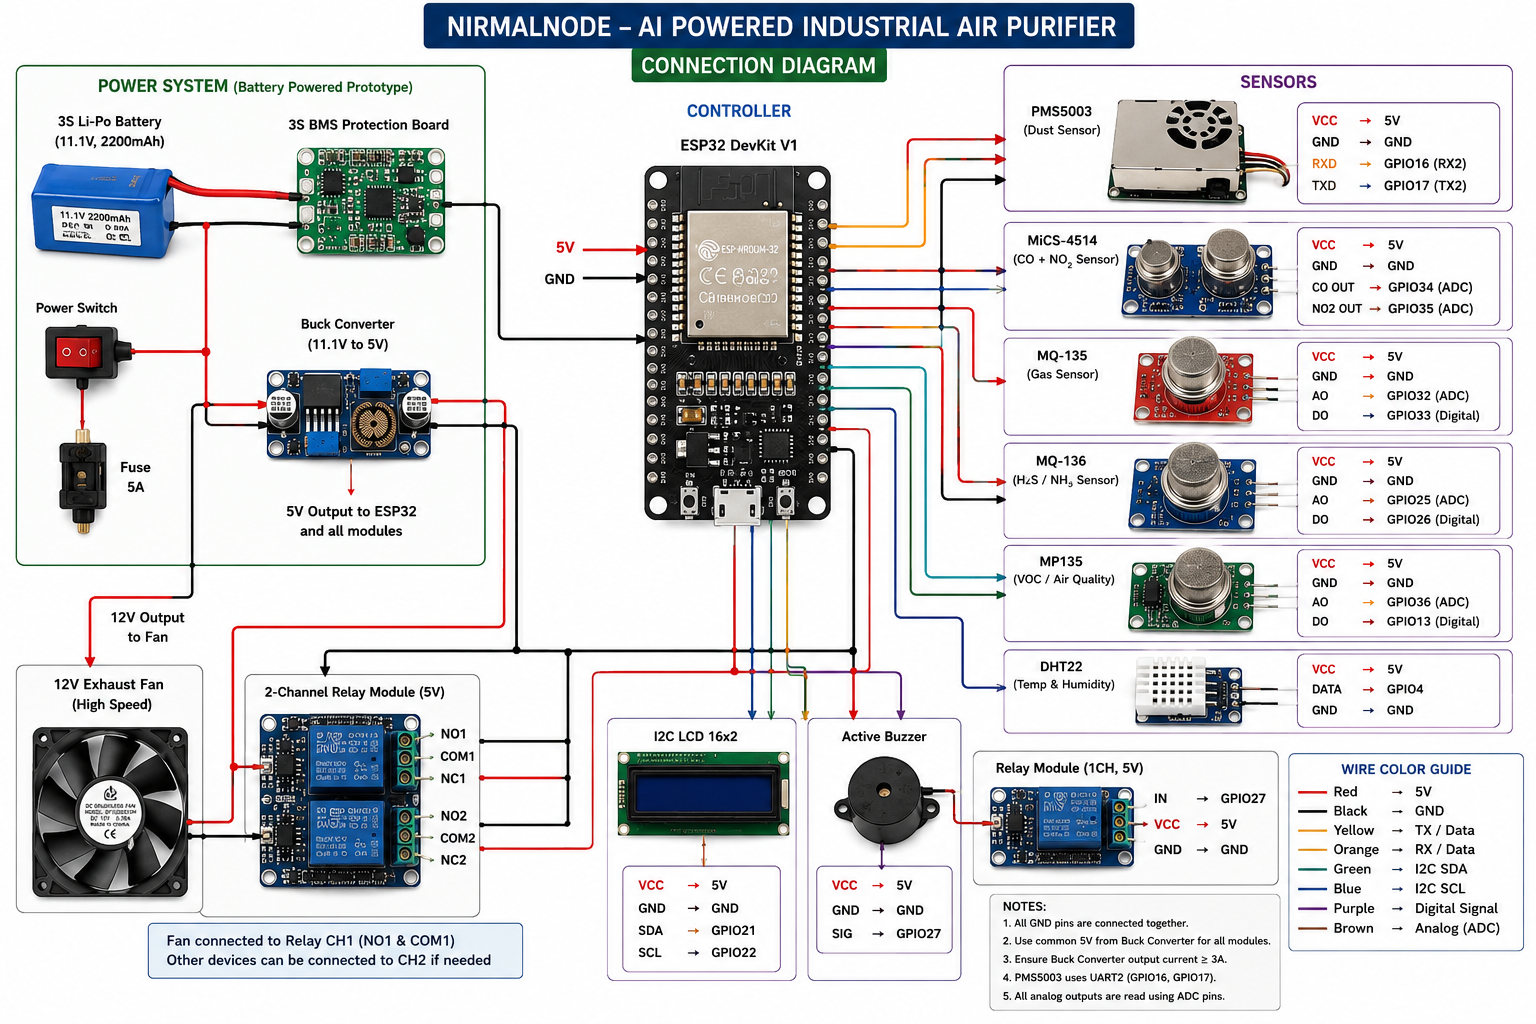
\includegraphics[width=0.92\textwidth]{figures/hardware_block_diagram.png}
\caption{Hardware block diagram and sensor pinout interfaces of a single NirmalNode unit.}
\label{fig:hardware-block}
\end{figure}

\FloatBarrier

\subsection{Software Block Diagram}
Figure~\ref{fig:software-block} decomposes the system's software into its constituent modules, spanning the ESP32 firmware (device-side) and the cloud service (server-side).

\begin{figure}[htbp]
    \centering
    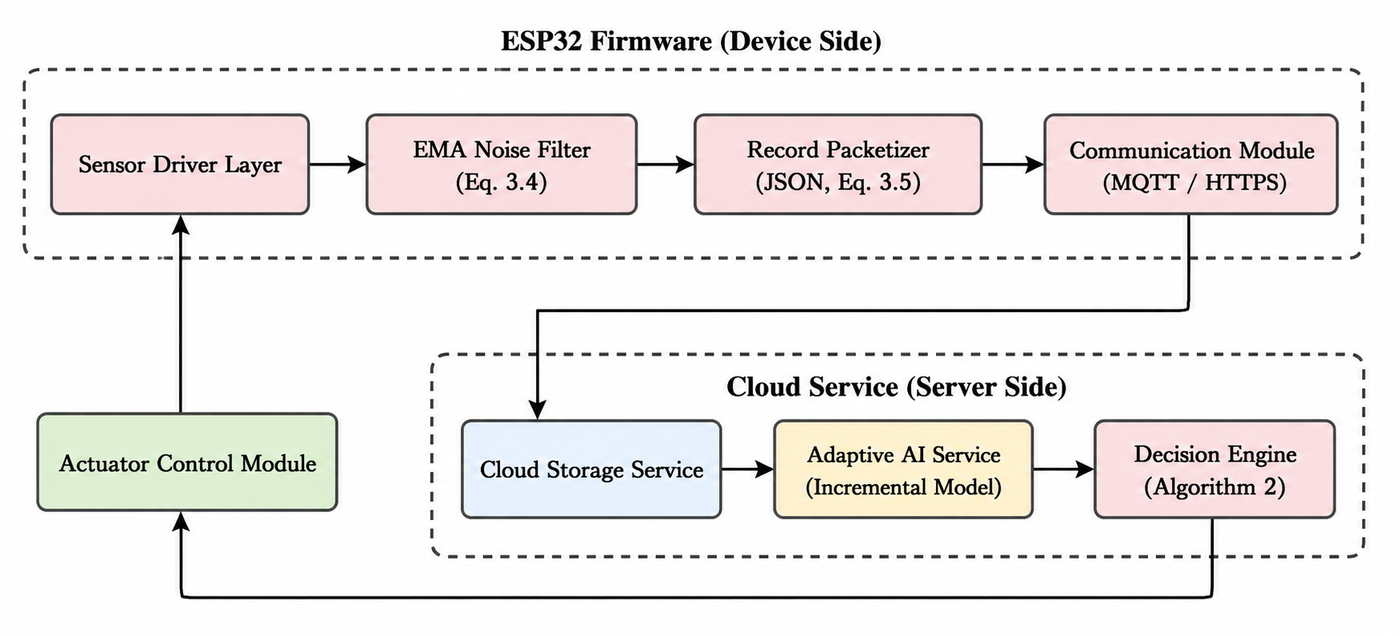
\includegraphics[width=\textwidth]{figures/software_block_diagram.png}
    \caption{Software block diagram, spanning device-side firmware and server-side cloud service.}
    \label{fig:software-block}
\end{figure}

\FloatBarrier

\subsection{AI Pipeline Diagram}
Figure~\ref{fig:ai-pipeline} illustrates the complete AI pipeline, from historical pre-training through continuous incremental updating and Model Arena election, described mathematically in Section~\ref{sec:meth-ai-pipeline}.

\begin{figure}[htbp]
\centering

\includegraphics[width=0.92\textwidth]{figures/ai_model_arena_pipeline.png}
\caption{AI pipeline: from historical pre-training to continuous incremental updating and Model Arena election.}
\label{fig:ai-pipeline}
\end{figure}

\FloatBarrier

\subsection{Incremental Learning Pipeline}
Figure~\ref{fig:incremental-pipeline} details the prequential (test-then-train) loop that gives NirmalNode its Adaptive AI and area-specific-learning properties, as introduced conceptually in Section~\ref{sec:lr-adaptive-ai}.

\begin{figure}[htbp]
\centering

\includegraphics[width=0.72\textwidth]{figures/incremental_learning_pipeline.png}
\caption{Incremental (online) learning pipeline, including area-specific re-adaptation on relocation or concept drift.}
\label{fig:incremental-pipeline}
\end{figure}

\FloatBarrier

\subsection{Purifier Decision Flowchart}
Figure~\ref{fig:decision-flowchart} presents the threshold-based purifier decision logic of Section~\ref{sec:meth-decision} (Equation~\ref{eq:decision-rule}, Algorithm~\ref{alg:decision-engine}) as a visual flowchart.

\begin{figure}[htbp]
\centering
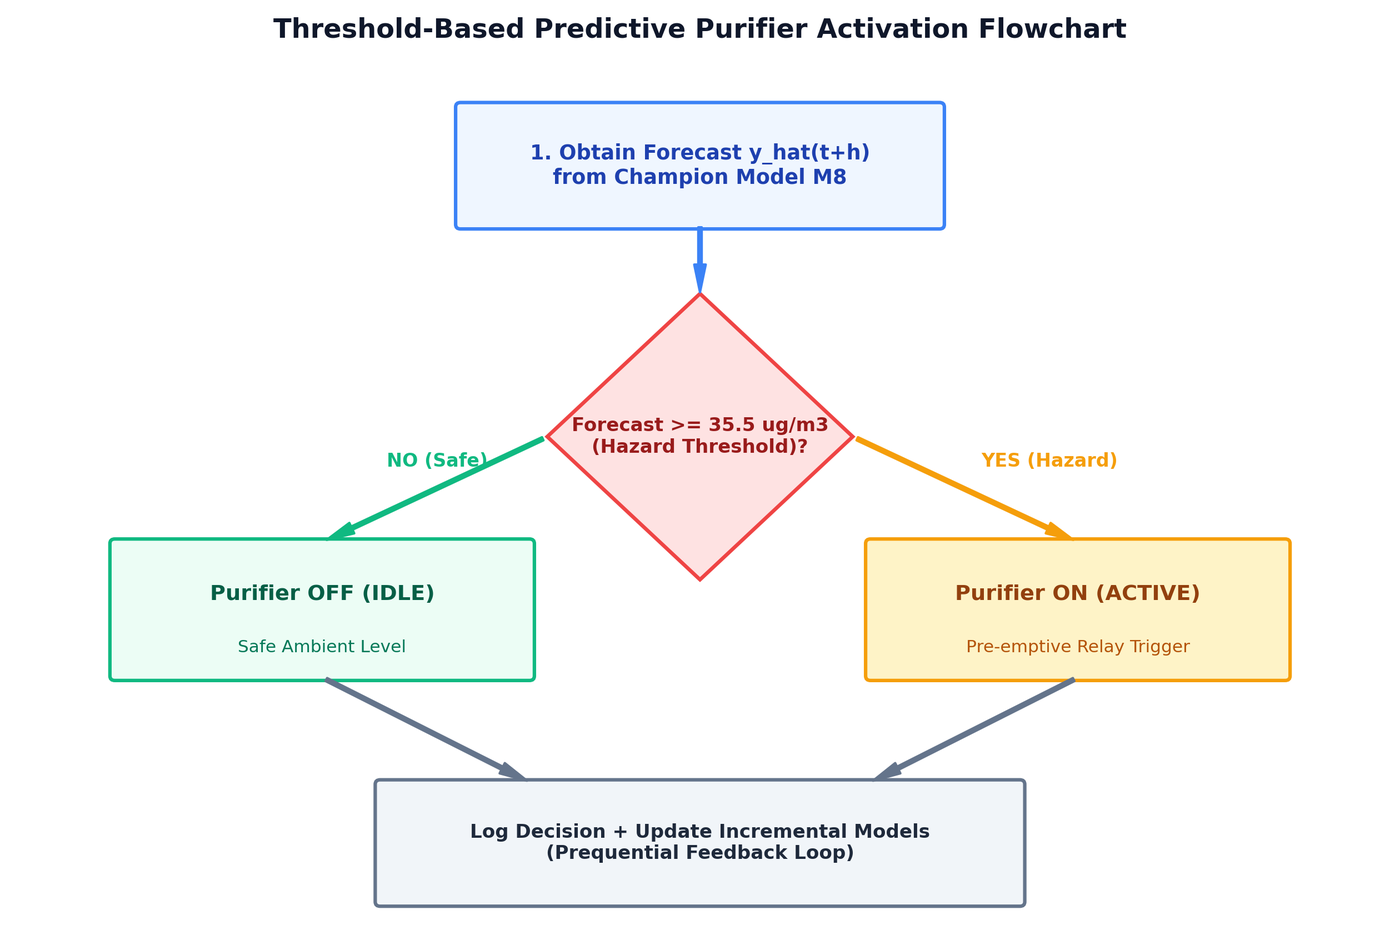
\includegraphics[width=0.78\textwidth]{figures/purifier_decision_flowchart.png}
\caption{Purifier decision flowchart: threshold-based pre-emptive activation and model update.}
\label{fig:decision-flowchart}
\end{figure}

\FloatBarrier

\subsection{Deployment Architecture}
Figure~\ref{fig:deployment-arch} shows how multiple NirmalNode units are envisaged to be deployed across the distinct hotspots of a single factory, each reporting independently to the shared cloud layer of Figure~\ref{fig:cloud-arch}, consistent with the multi-node future-work direction outlined in Section~\ref{sec:future-smartcity}.

\begin{figure}[htbp]
\centering
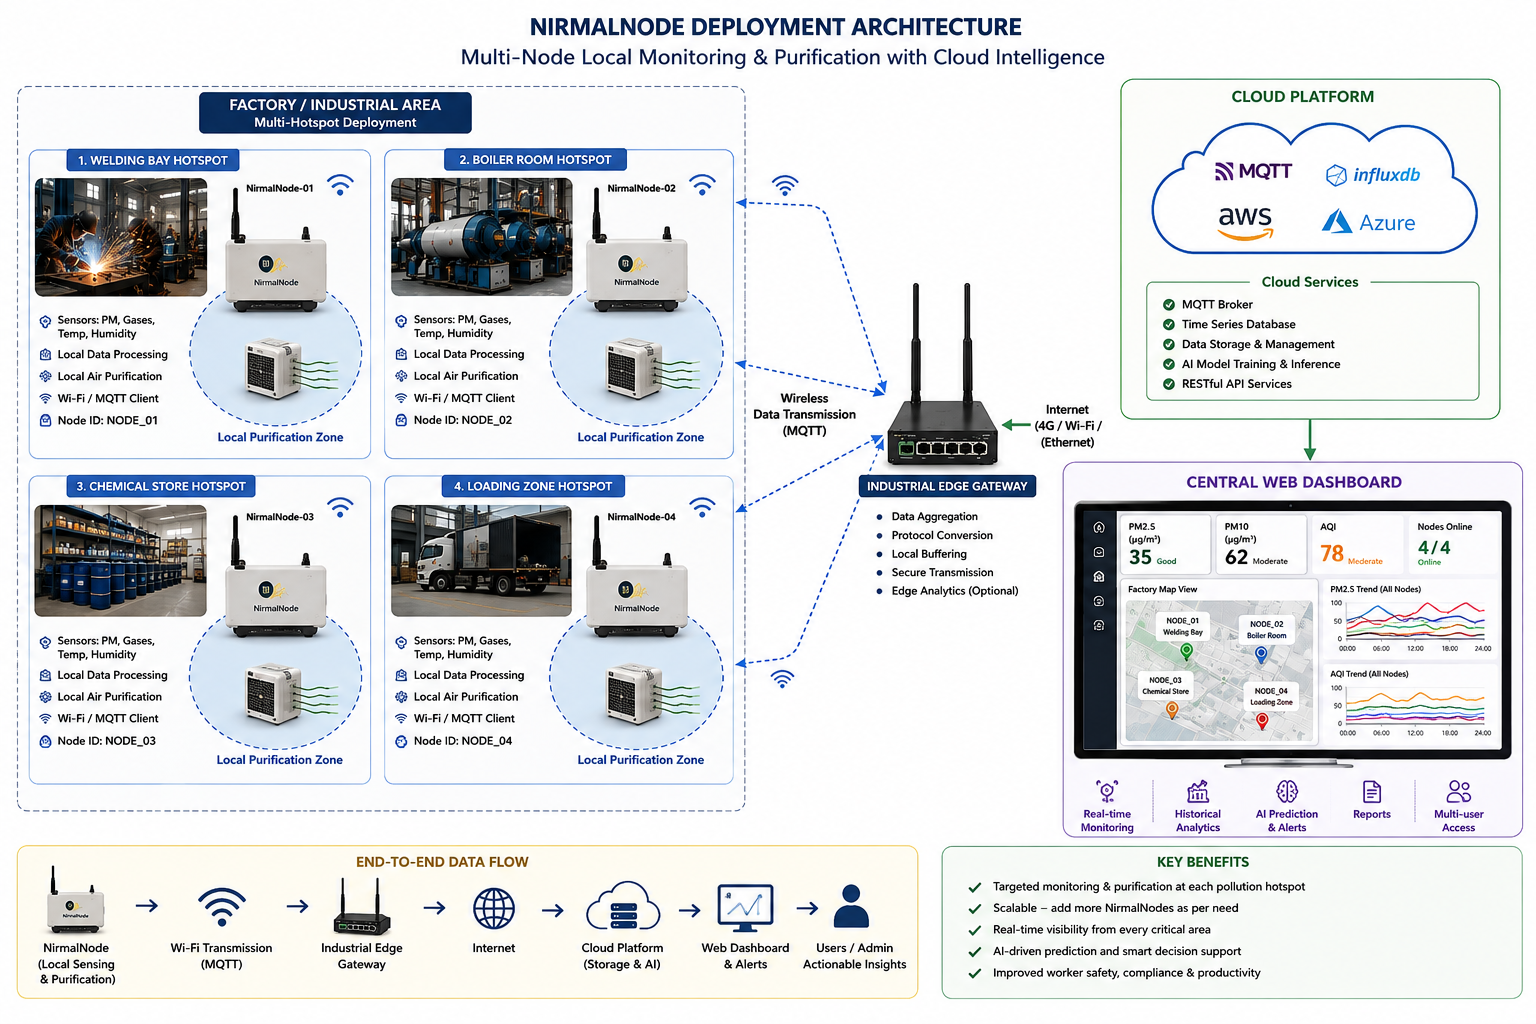
\includegraphics[width=0.92\textwidth]{figures/deployment_architecture.png}
\caption{Deployment architecture: multiple NirmalNode units across a factory's pollution hotspots, sharing a common cloud platform.}
\label{fig:deployment-arch}
\end{figure}

\FloatBarrier

\section{Explainable AI (XAI) Module}
\label{sec:meth-xai}

\subsection{Motivation}
\label{sec:meth-xai-motivation}

A central concern in safety-critical AI systems is \emph{interpretability}: the ability to explain \emph{why} the model made a specific prediction, not merely \emph{what} it predicted. For NirmalNode, interpretability is operationally important: a factory supervisor who receives a ``purifier ON'' command should be able to see which sensor readings drove the AI's decision, so they can (a) validate that the activation is physically plausible, (b) identify malfunctioning sensors whose anomalous readings are distorting the forecast, and (c) build confidence in the system over time. The XAI module added in this thesis addresses this need with two complementary explanations: \textbf{local} (per-prediction) feature contributions and \textbf{global} (all-time) feature importance.

\subsection{Method: Linear Feature Contribution (LFC)}
\label{sec:meth-xai-lfc}

For a linear model with learned weight vector $\mathbf{w} \in \mathbb{R}^d$ and bias $b$, the prediction is:
\begin{equation}
\hat{y} = \mathbf{w}^\top \tilde{\mathbf{x}} + b = \sum_{i=1}^{d} w_i \tilde{x}_i + b
\label{eq:linear-pred}
\end{equation}
where $\tilde{\mathbf{x}}$ is the standardized (zero-mean, unit-variance) feature vector. The \textbf{Linear Feature Contribution (LFC)} of feature $i$ to prediction $\hat{y}$ is therefore:
\begin{equation}
\phi_i = w_i \cdot \tilde{x}_i
\label{eq:lfc}
\end{equation}
such that $\hat{y} = b + \sum_{i=1}^{d} \phi_i$. The contributions are \textbf{exact} (not approximate): they sum to the prediction minus the bias term, and each $\phi_i$ directly measures how much feature $i$, at its current standardized value $\tilde{x}_i$, shifts the forecast up ($\phi_i > 0$) or down ($\phi_i < 0$) relative to the baseline. It can be shown that this is mathematically equivalent to the SHAP (SHapley Additive exPlanations) value for linear models \citep{lundberg2017shap}, making LFC the \emph{exact} SHAP solution without requiring the permutation-sampling approximation used for non-linear models.

For the NirmalNode blended SGD+PA model, the effective weight vector is:
\begin{equation}
\mathbf{w}_{\mathrm{blend}} = 0.6 \cdot \mathbf{w}_{\mathrm{SGD}} + 0.4 \cdot \mathbf{w}_{\mathrm{PA}}
\label{eq:blend-weight}
\end{equation}
and the LFC is computed using $\mathbf{w}_{\mathrm{blend}}$ in Equation~\ref{eq:lfc}.

\subsection{Global Feature Importance}
\label{sec:meth-xai-global}

The \textbf{global feature importance} of feature $i$ is defined as the magnitude of its blended learned weight, normalized across all $d = 14$ features:
\begin{equation}
I_i = \frac{|w_{\mathrm{blend},i}|}{\sum_{j=1}^{d} |w_{\mathrm{blend},j}|}
\label{eq:global-importance}
\end{equation}
$I_i \in [0,1]$ and $\sum_i I_i = 1$. Unlike the local LFC, global importance is independent of the current sample; it reflects which features the model has \emph{learned} to rely on most heavily across all training samples seen so far, and is thus a property of the model's current state rather than of any individual prediction.

\subsection{XAI Implementation}
\label{sec:meth-xai-impl}

The XAI module is implemented in the \texttt{AdaptiveAIEngine} class (\texttt{nirmal\_ml\_engine.py}) with the following methods:

\begin{itemize}
    \item \texttt{explain\_prediction(X\_sc)}: Computes per-feature LFC values from Equation~\ref{eq:lfc} for the most recently processed sample. Returns a list of dicts sorted by $|\phi_i|$ descending, each containing the feature name, raw value, contribution, and direction (``up'' / ``down'').
    \item \texttt{get\_global\_importance()}: Computes normalized global importance from Equation~\ref{eq:global-importance} using the current $\mathbf{w}_{\mathrm{blend}}$.
    \item \texttt{get\_shap\_explanation()}: Optional offline SHAP explanation using \texttt{shap.LinearExplainer} (requires \texttt{pip install shap}); uses the last $n$ history samples as the background distribution. Returns SHAP values and the expected value (base rate).
\end{itemize}

Algorithm~\ref{alg:xai} summarizes the per-sample XAI computation embedded in
\texttt{process\_stream\_sample()}:

\begin{algorithm}[htbp]
\caption{Per-sample LFC Explainability (appended to Algorithm~\ref{alg:decision-engine})}
\label{alg:xai}
\begin{algorithmic}[1]
\Require Blended weight vector $\mathbf{w}_{\mathrm{blend}}$, standardized feature vector $\tilde{\mathbf{x}}$
\State $\boldsymbol{\phi} \gets \mathbf{w}_{\mathrm{blend}} \odot \tilde{\mathbf{x}}$ \Comment{element-wise product, Eq.~\ref{eq:lfc}}
\State $\mathcal{R} \gets \{(i, \phi_i, \mathrm{sign}(\phi_i)) : i = 1,\ldots,d\}$ \Comment{feature name, contribution, direction}
\State Sort $\mathcal{R}$ by $|\phi_i|$ descending
\State \Return top-5 entries of $\mathcal{R}$ (for dashboard) + full $\mathcal{R}$ (for \texttt{/api/explain})
\end{algorithmic}
\end{algorithm}

\subsection{XAI Dashboard Integration}
\label{sec:meth-xai-dashboard}

The XAI module is exposed to the web dashboard through two mechanisms:

\begin{enumerate}
    \item \textbf{Per-prediction (local):} The top-5 LFC features are embedded in the \texttt{/api/ingest} response JSON under the \texttt{xai.top\_features} key, so the dashboard receives a fresh local explanation with every 2-second sensor update without an additional API call.
    \item \textbf{Global view:} A dedicated \texttt{/api/explain} REST endpoint returns the full global importance ranking, plus the complete 14-feature local contribution list for the most recent sample. The dashboard's ``Global Importance'' button fetches this endpoint on demand.
\end{enumerate}

The dashboard renders both views as animated horizontal bar charts (Figure~\ref{fig:xai-dashboard-screenshot}). Features with positive contributions ($\phi_i > 0$, pushing the forecast toward higher pollution) are shown in red bars growing rightward from the center; features with negative contributions ($\phi_i < 0$, pushing the forecast toward lower pollution) are shown in green bars growing leftward. Bar lengths are proportional to $|\phi_i|$ within each view.

\begin{table}[htbp]
\centering
\caption{Example local LFC explanation for a high-pollution sample (PM2.5 = 78~$\mu$g/m$^3$, 30 training samples)}
\label{tab:xai-example}
\small
\begin{tabular}{@{}lccl@{}}
\toprule
\textbf{Feature} & \textbf{Raw Value} & \textbf{Contribution $\phi_i$} & \textbf{Direction} \\
\midrule
PM2.5 delta (lag-1) & $+$48.0 & $-$27.80 & \textbf{Down} (sudden spike vs.\ low baseline) \\
PM2.5 EMA           & 28.4    & $+$15.47 & Up   (smoothed trend rising) \\
Count $>$2.5~$\mu$m & 58      & $+$14.65 & Up   (coarse-fraction count elevated) \\
PM10                & 113     & $+$14.10 & Up   (total particle mass high) \\
PM2.5 (current)     & 78      & $+$13.76 & Up   (current reading high) \\
\bottomrule
\end{tabular}
\end{table}

\noindent Table~\ref{tab:xai-example} shows a representative explanation: the model correctly identifies PM2.5, PM10, and particle counts as forecast-raising features, while the large negative lag-1 delta (the sudden jump from a low baseline) partially counteracts them -- an intuitively sensible decomposition that a non-expert supervisor can read and verify.

\FloatBarrier

\needspace{8\baselineskip}
\section{Chapter Summary}
\label{sec:meth-summary}

This chapter has presented the full NirmalNode methodology: a five-layer system architecture; hardware comprising an ESP32 controller, a PMS5003 particulate sensor, MQ135/MQ136/MiCS-4514/MP135 gas sensors, an optional BME280 environmental sensor, and a cyclone--HEPA--activated-carbon purification train; an EMA-filtered sensing firmware loop; an MQTT/HTTPS-based edge--cloud communication and storage architecture; an Adaptive AI pipeline built on incremental-learning estimators (SGD Regressor, Passive-Aggressive Regressor) that update continuously and adapt to new deployment areas without full retraining; a threshold-based Decision Engine that converts a 1--2 hour-ahead pollution forecast into a predictive, rather than reactive, purifier activation command; and an Explainable AI (XAI) module using Linear Feature Contribution (LFC) to provide transparent, per-prediction and global feature-importance explanations. Chapter 4 now describes the experimental setup used to evaluate this methodology and presents the corresponding results.

